\documentclass[a4paper,12pt,openany, DIV=calc]{scrbook}
\usepackage[utf8]{inputenc}
%\usepackage[cp1250]{inputenc}
\usepackage[T1]{fontenc}
\usepackage[polish]{babel}
%\usepackage[fixlanguage]{babelbib}
%\selectbiblanguage{polish}
%\usepackage[T1]{polski}
%\usepackage{times}
\usepackage{amsmath}
%\usepackage{amssymb}
\usepackage{amsfonts}
\usepackage{amsthm}
\usepackage{lmodern}
%\usepackage{scrpage2}
\usepackage{natbib}
\usepackage{float}

\usepackage{graphicx}
\usepackage{geometry}
\usepackage[pdftex]{hyperref}
%\usepackage{subfigure}
%\usepackage{longtable}
%\usepackage{stmaryrd}
%\usepackage{wasysym}
%\usepackage{lscape}
\usepackage{url}
%\usepackage{calc}
%\usepackage{multirow}
%\usepackage{multicol}
\usepackage{enumerate}
\usepackage{makeidx}
%\usepackage{epstopdf}
\usepackage{setspace}
\newgeometry{tmargin=1.5cm, bmargin=1.5cm, lmargin=2cm, rmargin=2cm}
\doublespacing
\addcontentsline{toc}{chapter}{Wstęp}
%\singlespacing
\begin{titlepage}
\titlehead{\center{\LARGE Uniwersytet Ekonomiczny w Krakowie}\\
\vskip2mm
{\LARGE Wydział Zarządzania}\\
\vskip2mm
{\LARGE Katedra Statystyki}}

\author{{\LARGE \textbf{Zygmunt Zawadzki}}\\
numer albumu: 161509\\
Kierunek: Analityka Gospodarcza\\
Specjalność: Modelowanie i Prognozowanie}

\subject{Praca magisterska}
\title{Filtracja danych wysokiej częstotliwości}
%\dedication{Rodzicom}
%\subtitle{Short but sweet?}
\publishers{{\Large Opiekun naukowy: dr hab. Daniel Kosiorowski}}
\vskip2mm
\date{Kraków, 2015}
\end{titlepage}
\begin{document}

\maketitle

\tableofcontents
\chapter*{Wstęp}


\chapter{Wprowadzenie}

Jednym z pobocznych celów tej pracy jest propozycja terminologii związanej z filtrowaniem HFFD

\begin{itemize}

\item[Bid] - cena po której otwierane są zlecenia sprzedaży i zamykane zlecenia kupna.
\item[Ask] - cena po której zamykane są zlecenia sprzedaży i otwierane zlecenia kupna.
\item[Mid] - średnia cen bid i ask.
\item[tick] - nowa obserwacja zmieniająca cenę Bid, lub Ask.
\item[spread] - różnica pomiędzy ceną kupna (Ask), a ceną sprzedaży (Bid).
\end{itemize}

\chapter{Charakterystyka danych wysokiej częstotliwości}

\subsection{Brak ciągłości w danych}.

\chapter{Projekt filtra}

\section{Potencjalne problemy}

\subsection{Zakleszczenie się filtra}

Bardzo niebezpieczną sytuacją do której może dojść jest odrzucanie przez filtr wszystkich nadchodzących danych (sytuację prezentuje \ref{fig:Kleszcze}). Takie zjawisko w dalszej części pracy będzie nazywane 'zakleszczeniem' się filtru.

\begin{figure}[H]
\centering
\begin{minipage}[t]{.47\textwidth}
  \centering
  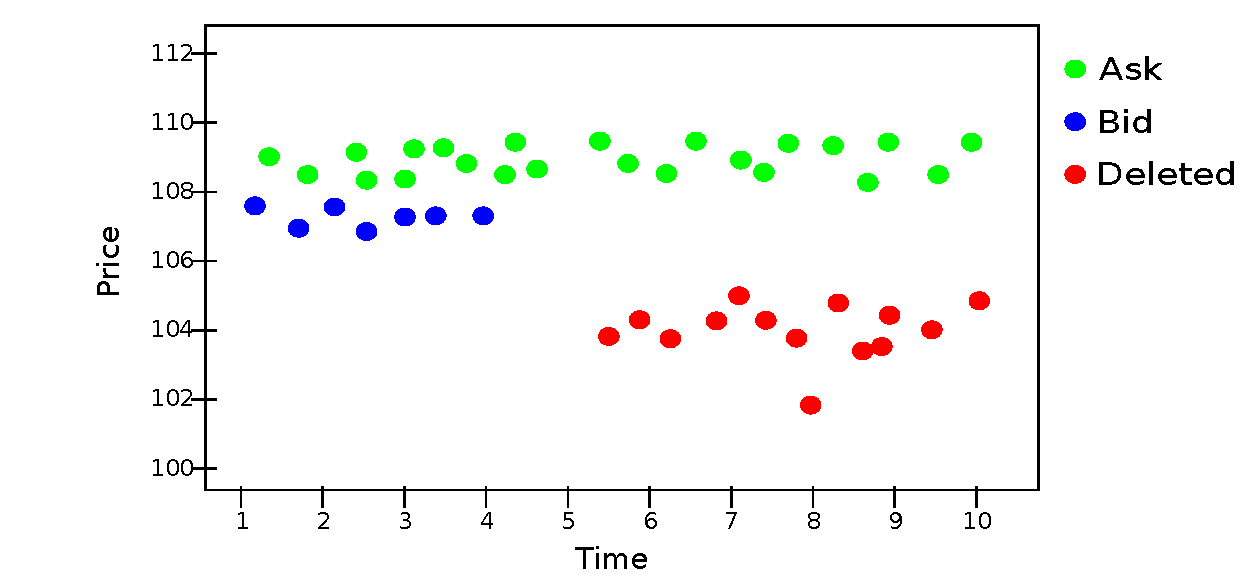
\includegraphics[width=\textwidth]{wykresy/kleszcze.pdf}
  \caption{Przypadel zakleszczenia się filtru. Po nagłym zwiększeniu się spreadu wszystkie kolejne ceny Bid są usuwane.}
  \label{fig:Kleszcze}
\end{minipage}%
\mbox{\hspace{0.1cm}} % To get a little bit of space between the figures
\begin{minipage}[t]{.47\textwidth}
  \centering
  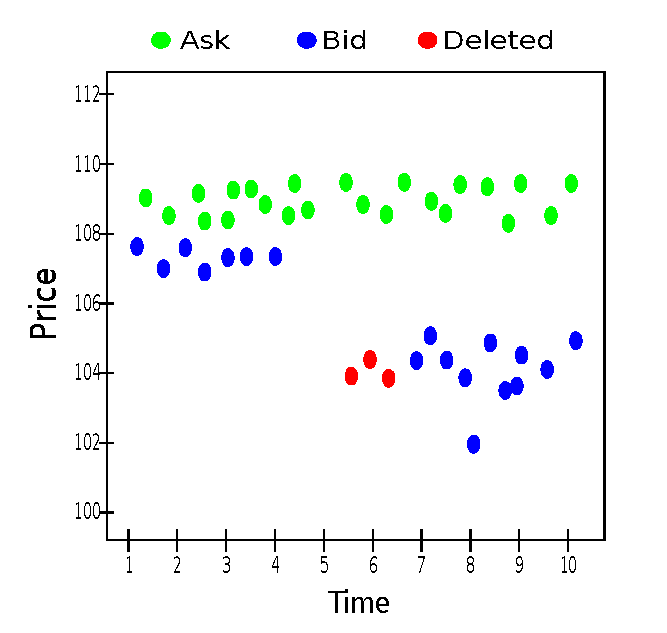
\includegraphics[width=\textwidth]{wykresy/kleszczeOK.pdf}
  \caption{Oczekiwane zachowanie filtra. Tylko część prawidłowych ticków zostaje usunięta.}
  \label{fig:KleszczeOK}
\end{minipage}

\end{figure}



\subsection{Relacja pomiędzy ceną Bid i Ask}

\begin{figure}[H]
  \centering
  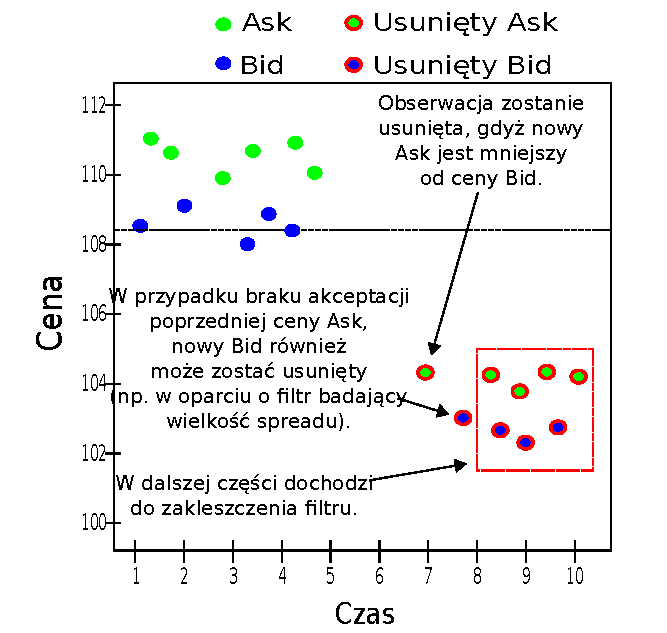
\includegraphics[width=0.6\textwidth]{wykresy/relacjaBIDASK.pdf}
  \caption{Przypadel zakleszczenia się filtru. Po nagłym zwiększeniu się spreadu wszystkie kolejne ticki są usuwane.}
  \label{fig:BIDASK}

\end{figure}

\subsection{Długa seria złych ticków}


\bibliographystyle{plainnat}
\bibliography{literatura_mag}
\addcontentsline{toc}{section}{Bibliografia}
\listoftables
\addcontentsline{toc}{section}{Spis tabel}
\listoffigures
\addcontentsline{toc}{section}{Spis rysunków}
\printindex
\end{document}
